\subsubsection{\emph{Logical View}}
\label{subsubsec:logical-view}

\begin{figure}[htbp]
    \centering
    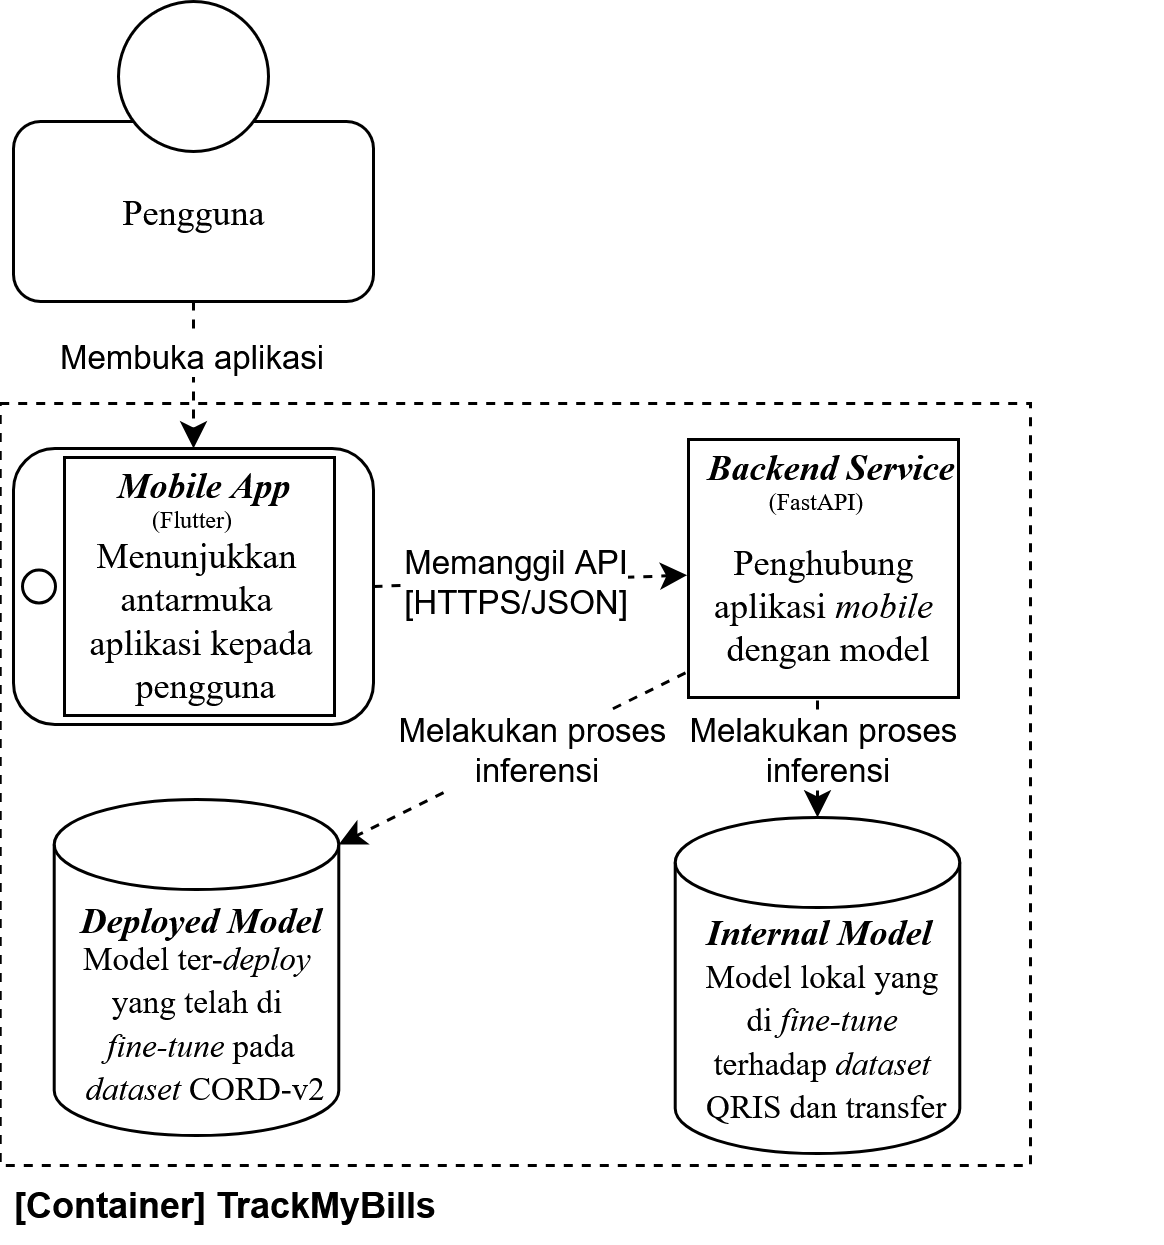
\includegraphics[width=.8\textwidth]{images/container-diagram.png}
    \caption{\emph{Container diagram} sistem pencatatan pengeluaran berbasis \emph{mobile}}
    \label{fig:container-diagram}
\end{figure}

\emph{Logical view} menggambarkan struktur sistem dari sudut pandang logis dari entitas-entitas yang ada dalam sistem secara konseptual. \autoref{fig:container-diagram} menunjukkan \emph{container diagram} sistem pencatatan pengeluaran berbasis \emph{mobile}. Diagram ini menunjukkan bagaimana sistem dibagi menjadi beberapa kontainer, yaitu aplikasi \emph{mobile}, layanan \emph{backend}, model internal, dan model \emph{deployed}. Setiap kontainer memiliki tanggung jawab dan interaksi yang jelas, yang memungkinkan pengembangan dan pemeliharaan sistem menjadi lebih terstruktur.

\autoref{fig:container-diagram} menunjukkan pengguna yang akan berinteraksi dengan aplikasi \emph{mobile}. Aplikasi \emph{mobile} berkomunikasi dengan layanan \emph{backend} melalui API, yang memungkinkan aplikasi untuk mengirim dan menerima data melalui protokol HTTP/JSON. Layanan \emph{backend} bertanggung jawab untuk memproses data dan menghubungkan dengan model internal dan model \emph{deployed}. Model internal dan model \emph{deployed} berfungsi untuk melakukan inferensi dari data yang diterima dari layanan \emph{backend}.


